\documentclass[11pt,a4paper]{article}
\usepackage[utf8]{inputenc}
\usepackage[english]{babel}
\usepackage[left=1.5cm,right=1.5cm,top=1.5cm,bottom=1.5cm]{geometry}
\author{Andreas Hemmetter}
\let\footruleskip\undefined %undefine footruleskip
\usepackage{fancyhdr}
\usepackage{multicol}
\usepackage{microtype}
% \usepackage{textcomp}
% \usepackage{amsthm}
\usepackage{framed}
\usepackage{multirow}
\usepackage{xhfill}
\usepackage{makecell}
% \usepackage{bbold}
% \usepackage{amssymb}
\usepackage{hyperref}
\usepackage{booktabs}
\usepackage{graphicx}
\usepackage{setspace}
\usepackage{lettrine}
%\usepackage{braket}
% \usepackage{tikz}
% \usetikzlibrary{arrows}
\usepackage[sorting=none]{biblatex}
\addbibresource{refs.bib}
\AtBeginBibliography{\small} 
\definecolor{shadecolor}{rgb}{0.95, 0.95, 0.95}

\setlength{\headheight}{15.2pt}
\begin{document}
\pagestyle{fancyplain}
\fancyhf{}
\rhead{\textbf{\textit{A World Federation}} - \href{mailto:ahemmetter@gmail.com}{A. Hemmetter} }
\rfoot{\scriptsize{This work is licensed under a \href{https://creativecommons.org/licenses/by-sa/4.0/}{Creative Commons Attribution-ShareAlike 4.0 International License}.}}
\begin{center}

\begin{tabular}[t]{@{}l}
\rule[4pt]{0.22\linewidth}{4pt}
\end{tabular}
\begin{tabular}[t]{@{}}
\fontsize{24pt}{10pt}
\textbf{A World Federation}
\end{tabular}
\begin{tabular}[t]{r@{}}
\rule[4pt]{0.22\linewidth}{4pt}
\end{tabular}
\end{center}

\begin{multicols}{2}
\lettrine[lraise=0.1, lines=2]{\textsc{H}}{umans} have built civilization for over 12 000 years. Through science, art, philosophy, technology and hard work we have catapulted ourselves into an entirely new world. Yet our political institutions have not caught up: we are still caught in the paradigms of the previous centuries.

\noindent Today, our world truly is a global village. Travel, the internet, markets and the nature weave an ever tighter web around us humans. In this interdependent world, nations have become too small to make a difference in dealing with our most serious problems. A democratically elected government for a world federation is our best shot at saving ourselves and unleashing humanity’s potential.


\begin{shaded*}
\noindent \textit{Till the war-drum throbbed no longer,\\
and the battle-flags were furled\\
\noindent In the Parliament of man, \\
the Federation of the world.}
%\vspace{-22pt}
\begin{flushright}
-- Alfred Tennyson
\end{flushright}
\vspace{-12pt}
\end{shaded*}


\paragraph{A Story of Unification}

Much of our collective history is a story of continuous unification.
From the tribes of the Stone Age to the founding of modern nations, our ancestors have united with former enemies into larger states.
They have formulated, interpreted and enforced the rule of law to ensure peace, prosperity and progress in the face of ever larger problems.\\
\noindent Peace is not just the absence of war, but rather the resolution of conflicts through the application of law.
Our nations, states, counties, communities and families diligently take on this duty every day.
Law, along with fire, the wheel, writing and electricity, has proven to be humanity's most successful inventions.
If you want peace, prepare the law.

\begin{shaded*}
\noindent \textit{A federation of all humanity, together with a sufficient means of social justice to ensure health, education, and a rough equality of opportunity, would mean such a release and increase of human energy as to open a new phase in human history.}
%\vspace{-22pt}
\begin{flushright}
-- H. G. Wells
\end{flushright}
\vspace{-12pt}
\end{shaded*}

\noindent Yet curiously, this universal principle yields to the idol of national sovereignty on the world state.
We hold this truth to be self evident: that my nation has absolute freedom to defend its interests.  
Who defends the interests of humanity?

\end{multicols}
\paragraph{Troubles Don't Respect Borders}

The world has changed. No longer are problems small enough to be solved by a country alone.
The threats we face today have no consideration for borders.\\
\noindent All people share the same atmosphere.
Greenhouse gases change our climate regardless of where the most has been emitted.
Even though the solutions are well known, nations are trapped by their economic competition in this anarchic world, unable to free themselves. \hfill Protocols are not enough.\\
\noindent Even after decades of foreign aid and donations, there are still too many people living under conditions we cannot justify.
Inadequate sanitation and international travel help the spread of infectious diseases to us.
Poverty and the lack of opportunities rekindle violence, corruption and drug and human trafficking and endanger our safety at home.
\hfill Aid is not enough.\\
\noindent Many of us have never had to experience war.
History has shown us that we cannot take this for granted, much less in a time of nuclear, biological and chemical weapons of mass destruction.
Of course, no one wants war, yet sometimes it becomes necessary to defend one's national freedom.
It is in fact the unrestrained national freedom itself that lies at the root of war.
Today, conflicts are resolved by power, whether assumed or unleashed.
The anarchy of sovereign states is a ticking time bomb. \hfill Pacifism is not enough.
\begin{multicols}{2}

\paragraph{Beyond Nations} 

Every single one of us understands what's at stake.
We look to governments for solutions, but fail to see relief come from them.
It is a tragedy that our world cannot take care of its common goods and interests.
We, the people of the world, need a democratic, federal world government, fit to guard and advance our world.

\noindent We need a public representation of all people on Earth that handles issues national governments cannot.
A majority of Earth's inhabitants would have the power to enforce action to end climate change, poverty and remove the causes of war.
The world can be sustainable without the fear of disadvantage.
The poorest can be lifted up and freed from exploitation.
Tensions can be resolved democratically, rather than through projected force.
Such a unity would release an awesome amount of human energy and open the door to a new era.

\paragraph{Federal Republic of Earth}

You might be frightened of the prospect of a powerful government.
Could it degrade into an oppressive regime?\\
\noindent Every nation faces the same risk.
We have found that healthy democratic institutions with a constitution safeguards a republic from abuse.
The lack of such institutions at the global level makes us powerless victims of the tyranny of planet-wide issues and the decisions of foreign countries.

\begin{shaded*}
\noindent \textit{Mankind's desire for peace can be realized only by the creation of a world government. With all my heart, I believe that the world's present system of sovereign nations can only lead to barbarism, war, and inhumanity.}
%\vspace{-11pt}
\begin{flushright}
-- Albert Einstein
\end{flushright}
\vspace{-12pt}
\end{shaded*}

\paragraph{United Nations}

From the shock of the last world war, we have created an assembly of states, the United Nations. What more could we want?\\
\noindent The United Nations provide an invaluable forum for governments to address their concerns and make proposals.
Yet the structure of the United Nations contains fundamental flaws that stop it from being effective.
People are represented only by their governments, disregarding internal public opinion or population size.
A single nuclear-armed nation can block any important resolution it desires.
Finally, the resolutions that do pass are toothless treaties; whether they are enforced is up to national governments in the end.
Time and time again the United Nations have failed to live up to the expectations put into them.
The United Nations are not a world government, but they are a stepping stone to one.


\paragraph{Utopia}

Despite the prospects, you might be discouraged, seeing how nations cling to their sovereignty.. What would it take to live in the Federal Republic of Earth?\\
\noindent Men who saw the devastation of war with their own eyes founded the United Nations. We are lucky to have a solid base which to improve on by incremental steps.
A world parliament, representing the people in a second legislative chamber next to the General Assembly, is a first step in the direction of world federation.
The Parliament and General Assembly together can pick a government that sets the course and the International Court of Justice and be given more than just advisory power to complete the triad of separated powers.

\begin{shaded*}
\noindent \textit{Unless some effective supranational government can be set up and brought quickly into action, the prospects of peace and human progress are dark and doubtful.}
%\vspace{-11pt}
\begin{flushright}
-- Winston Churchill
\end{flushright}
\vspace{-12pt}
\end{shaded*}

\end{multicols}

\paragraph{What Is to Be Done?}

This short pamphlet could not possibly convey the wealth of thought that has gone into the betterment of humanity by uniting it.
It can, however, point you to this wealth.
Below are some of the more concise explanations of the theory, necessity and implementation of a democratic world federation. Already many associations and communities have formed that have the goal of bringing about a unified world.
The Young World Federalists offer a lively community for discussion and action.
Exchange and develop your ideas!
Demand the change we deserve!
So that we can finally live in peace, prosperity and progress on this pale blue Earth.

\vspace{11pt}
\hline

\begin{multicols}{2}
\nocite{*}
\begingroup
\setstretch{0.8}
\setlength\bibitemsep{2pt}
\printbibliography[heading=none]
\endgroup
\end{multicols}

\begin{minipage}{.75\textwidth}
\begin{shaded*}
\begin{tabular}{r|l}
\makecell[r]{\large{\textbf{Young World}}\\ \large{\textbf{Federalists}}} & \makecell[l]{\textbf{\href{https://www.ywf.world}{ywf.world}} $\mid$ \textbf{\href{https://discord.gg/WyUkQps}{Discord}} $\mid$ \textbf{\href{https://twitter.com/ywf_world}{@ywf\_world}}\\  
\textbf{\href{https://www.reddit.com/r/GlobalTribe/}{r/GlobalTribe}} $\mid$ \textbf{\href{https://www.youtube.com/channel/UCBWca8XnMHF9EELWbz146pg}{YouTube}} $\mid$ \textbf{\href{https://www.facebook.com/YoungWorldFederalists/}{Facebook}}}
\end{tabular}

\end{shaded*}
\end{minipage}%
\begin{minipage}{0.25\textwidth}
\vspace{-30pt}
    \centering
    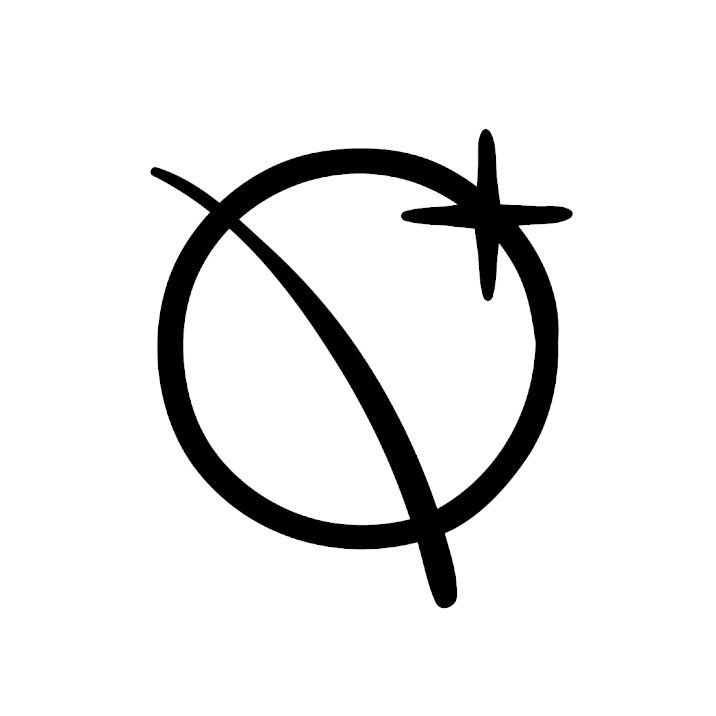
\includegraphics[height=100px]{ywf.png}

\end{minipage}

\end{document}
